\subsubsection{Rede Neural Artificial}

Uma rede neural artificial é uma representação matemática de unidades de processamento conectadas, chamadas de neurônios artificiais. Esta arquitetura simula sinapses; cada sinal trocado entre os neurônios pode aumentar ou atenuar os sinais de outros durante o aprendizado \cite{ml_and_dp}.

Observa-se na \cref{fig:neuronio} o funcionamento de um neurônio $k$. Os sinais de entrada são partes de um vetor $x$ de tamanho $n$, sendo o vetor composto por $x_1, x_2, \ldots, x_n$. Essas componentes são combinadas em uma soma ponderada utilizando seus respectivos pesos, $w_{k1}, w_{k2}, \ldots, w_{kn}$, formando assim a seguinte equação \apud{marti2017aprendizado}{haykin1999neural}:

\begin{figure}[ht]
	\centering
	\caption{Modelo de um neurônio não-linear.}
	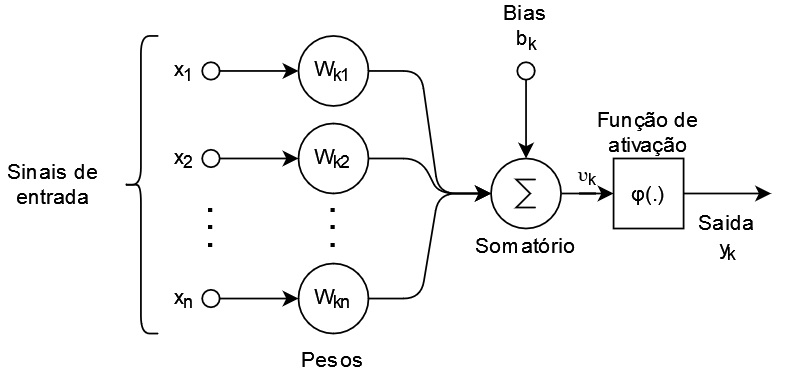
\includegraphics[width=0.8\textwidth]{figures/neuronio.png}
	\legend{Fonte: \citeonline{haykin1999neural}}
	\label{fig:neuronio}
\end{figure}

\begin{equation}
	\upsilon_k = \sum_{i=1}^n (x_i * w_{ki})
\end{equation}

O resultado dessa equação produz o potencial de ativação $\upsilon_k$, que, somado ao \textit{bias} ou viés $b_k$, manipula a saída $y_k$ do neurônio. Essa soma é colocada em uma função não-linear, nomeada de função de ativação $\varphi(.)$. Essas funções mapeiam a saída em um intervalo $[0, 1]$ ou $[-1, 1]$. A função de saída pode ser representada pela seguinte equação \apud{marti2017aprendizado}{haykin1999neural}:

\begin{equation}
	y_k = \varphi(\upsilon_k + b_k)
\end{equation}

O aprendizado ocorre na fase de treinamento, onde são ajustados os pesos $w_k$ e o viés $b_k$ de cada neurônio $k$. Os pesos $w_k$ são utilizados para calcular a taxa de crescimento da função, e o viés $b_k$ é necessário para deslocar a saída da função. Com isso, é possível modelar uma função linear $y = w^T x + b$ \cite{marti2017aprendizado}.

Para cada amostra, o modelo compara os resultados dos valores atuais dos pesos $w_k$ e viés $b_k$ com o resultado esperado (alvo). Uma função de perda é utilizada para gerar um vetor de gradientes e quantificar o erro encontrado na configuração atual do modelo. O modelo atualiza os pesos $w_k$ e os viés $b_k$ no sentido contrário do vetor de gradientes, buscando minimizar a função de perda de acordo com uma taxa de aprendizado (\textit{learning rate}). Esse processo é chamado de retropropagação ou \textit{backpropagation} \cite{marti2017aprendizado}.

Ao combinar diversos neurônios artificiais, forma-se uma rede neural artificial. Essas redes buscam simular o processamento de informação do cérebro humano \cite{ferneda2006redes}.

Nas redes neurais, os neurônios são organizados em grupos de unidades de processamento chamados camadas. A primeira e a última camadas são nomeadas de camada de entrada e camada de saída, respectivamente, e as demais são chamadas de camadas ocultas. As camadas mais próximas da entrada são responsáveis por identificar características mais primitivas, e as seguintes combinam essas informações para identificar padrões mais complexos \cite{marti2017aprendizado}.
